\documentclass[11pt]{article}
\usepackage[margin=1in]{geometry}
\usepackage{booktabs}
\usepackage{graphicx}
\usepackage{hyperref}
\usepackage{amsmath}

\title{Text as Data in Social Science:\\ A Systematic Review of the Evolution of Language-Based Methods from Content Analysis to Large Language Models (1916--2026)}
\author{Ann Naser Nabil}
\date{\today}

\begin{document}
\maketitle

\begin{abstract}
Text-as-data methods have moved from manual content analysis to dictionary scoring, supervised machine learning, topic models, transformers, and large language models. This paper develops a cross-disciplinary framework for understanding that evolution across economics, political science, communication, sociology, psychology, computational social science, and NLP-adjacent social research. The current draft implements a seed-review prototype based on 28 canonical papers from 1927 to 2026. It is not yet a completed PRISMA-style systematic review. The prototype demonstrates the coding scheme, historical periodization, method taxonomy, validation comparison, and LLM-era research agenda that will structure the final 200--400 paper review.
\end{abstract}

\section{Introduction}

Social scientists increasingly treat language as measurable data. Parliamentary speeches, newspaper articles, court opinions, survey responses, social media posts, central-bank statements, and online reviews are now routinely transformed into variables, indices, predictions, and qualitative summaries. Yet the field remains fragmented. Political scientists cite one methodological canon, economists cite another, communication scholars inherit content-analysis traditions, psychologists use dictionaries such as LIWC, and computational social scientists move quickly toward embeddings and large language models.

This review asks how language has been transformed into social-scientific evidence over roughly a century, and what the transition from manual coding to LLMs reveals about future research. The contribution is threefold. First, it provides a historical synthesis of text-as-data methods. Second, it proposes a unified taxonomy by method, task, data type, discipline, and validation standard. Third, it develops a research agenda for the LLM era, emphasizing validation, multilingual coverage, reproducibility, and low-resource contexts.

This draft is a prototype. It implements the review infrastructure using a curated seed database. The final version should expand this into a full systematic review with formal search logs, screening decisions, and a PRISMA diagram.

\section{Historical Eras}

The seed review uses seven historical eras. Table \ref{tab:eras} reports the number of seed papers coded into each era.

\begin{table}[ht]
\centering
\caption{Historical eras in the seed database}
\label{tab:eras}
\begin{tabular}{llr}
\toprule
era & era\_label & n \\
\midrule
content\_analysis\_1916\_1950 & Content analysis
1916-1950 & 2 \\
quant\_content\_1950\_1980 & Quant content
1950-1980 & 3 \\
computer\_assisted\_1980\_2000 & Computer-assisted
1980-2000 & 1 \\
dictionary\_2000\_2010 & Dictionaries
2000-2010 & 3 \\
topic\_ml\_2010\_2018 & Topics + ML
2010-2018 & 7 \\
transformers\_2018\_2022 & Transformers
2018-2022 & 5 \\
llm\_2022\_2026 & LLMs
2022-2026 & 7 \\
\bottomrule
\end{tabular}

\end{table}

\subsection{Era 1: Content Analysis, 1916--1950}

The earliest era treated text as evidence about propaganda, political persuasion, and mass communication. The method was manual and interpretive, but it established the idea that systematic analysis of language could reveal social and political structure.

\subsection{Era 2: Quantitative Content Analysis, 1950--1980}

The second era formalized coding schemes and reliability standards. The key methodological shift was not automation, but discipline: categories had to be explicit, coders had to be trained, and agreement had to be documented.

\subsection{Era 3: Computer-Assisted Text Analysis, 1980--2000}

Computer-assisted content analysis introduced concordances, keyword-in-context tools, and early dictionaries. The General Inquirer and related systems showed that machines could scale some forms of coding, although the conceptual categories still came from human researchers.

\subsection{Era 4: Dictionary Methods, 2000--2010}

Dictionary methods became widely used in psychology, economics, finance, and political communication. They offered transparency and low cost, but often struggled with context, negation, sarcasm, domain shift, and non-English language coverage.

\subsection{Era 5: Topic Models and Machine Learning, 2010--2018}

Topic models, supervised classifiers, and structural topic models changed the tasks social scientists could pursue. Researchers could discover themes, classify large corpora, and link text-derived quantities to institutional or economic outcomes.

\subsection{Era 6: Transformers and Embeddings, 2018--2022}

Transformer models shifted text-as-data from sparse word counts to contextual representations. This improved classification and semantic retrieval, but increased concerns about opacity, computational access, and reproducibility.

\subsection{Era 7: Large Language Models, 2022--2026}

LLMs changed the interface. Researchers can now prompt models to classify, summarize, annotate, translate, and simulate. This creates new possibilities, but it also exposes measurement risks: model drift, hidden training data, hallucination, inconsistent outputs, and uneven multilingual performance.

\begin{figure}[ht]
\centering
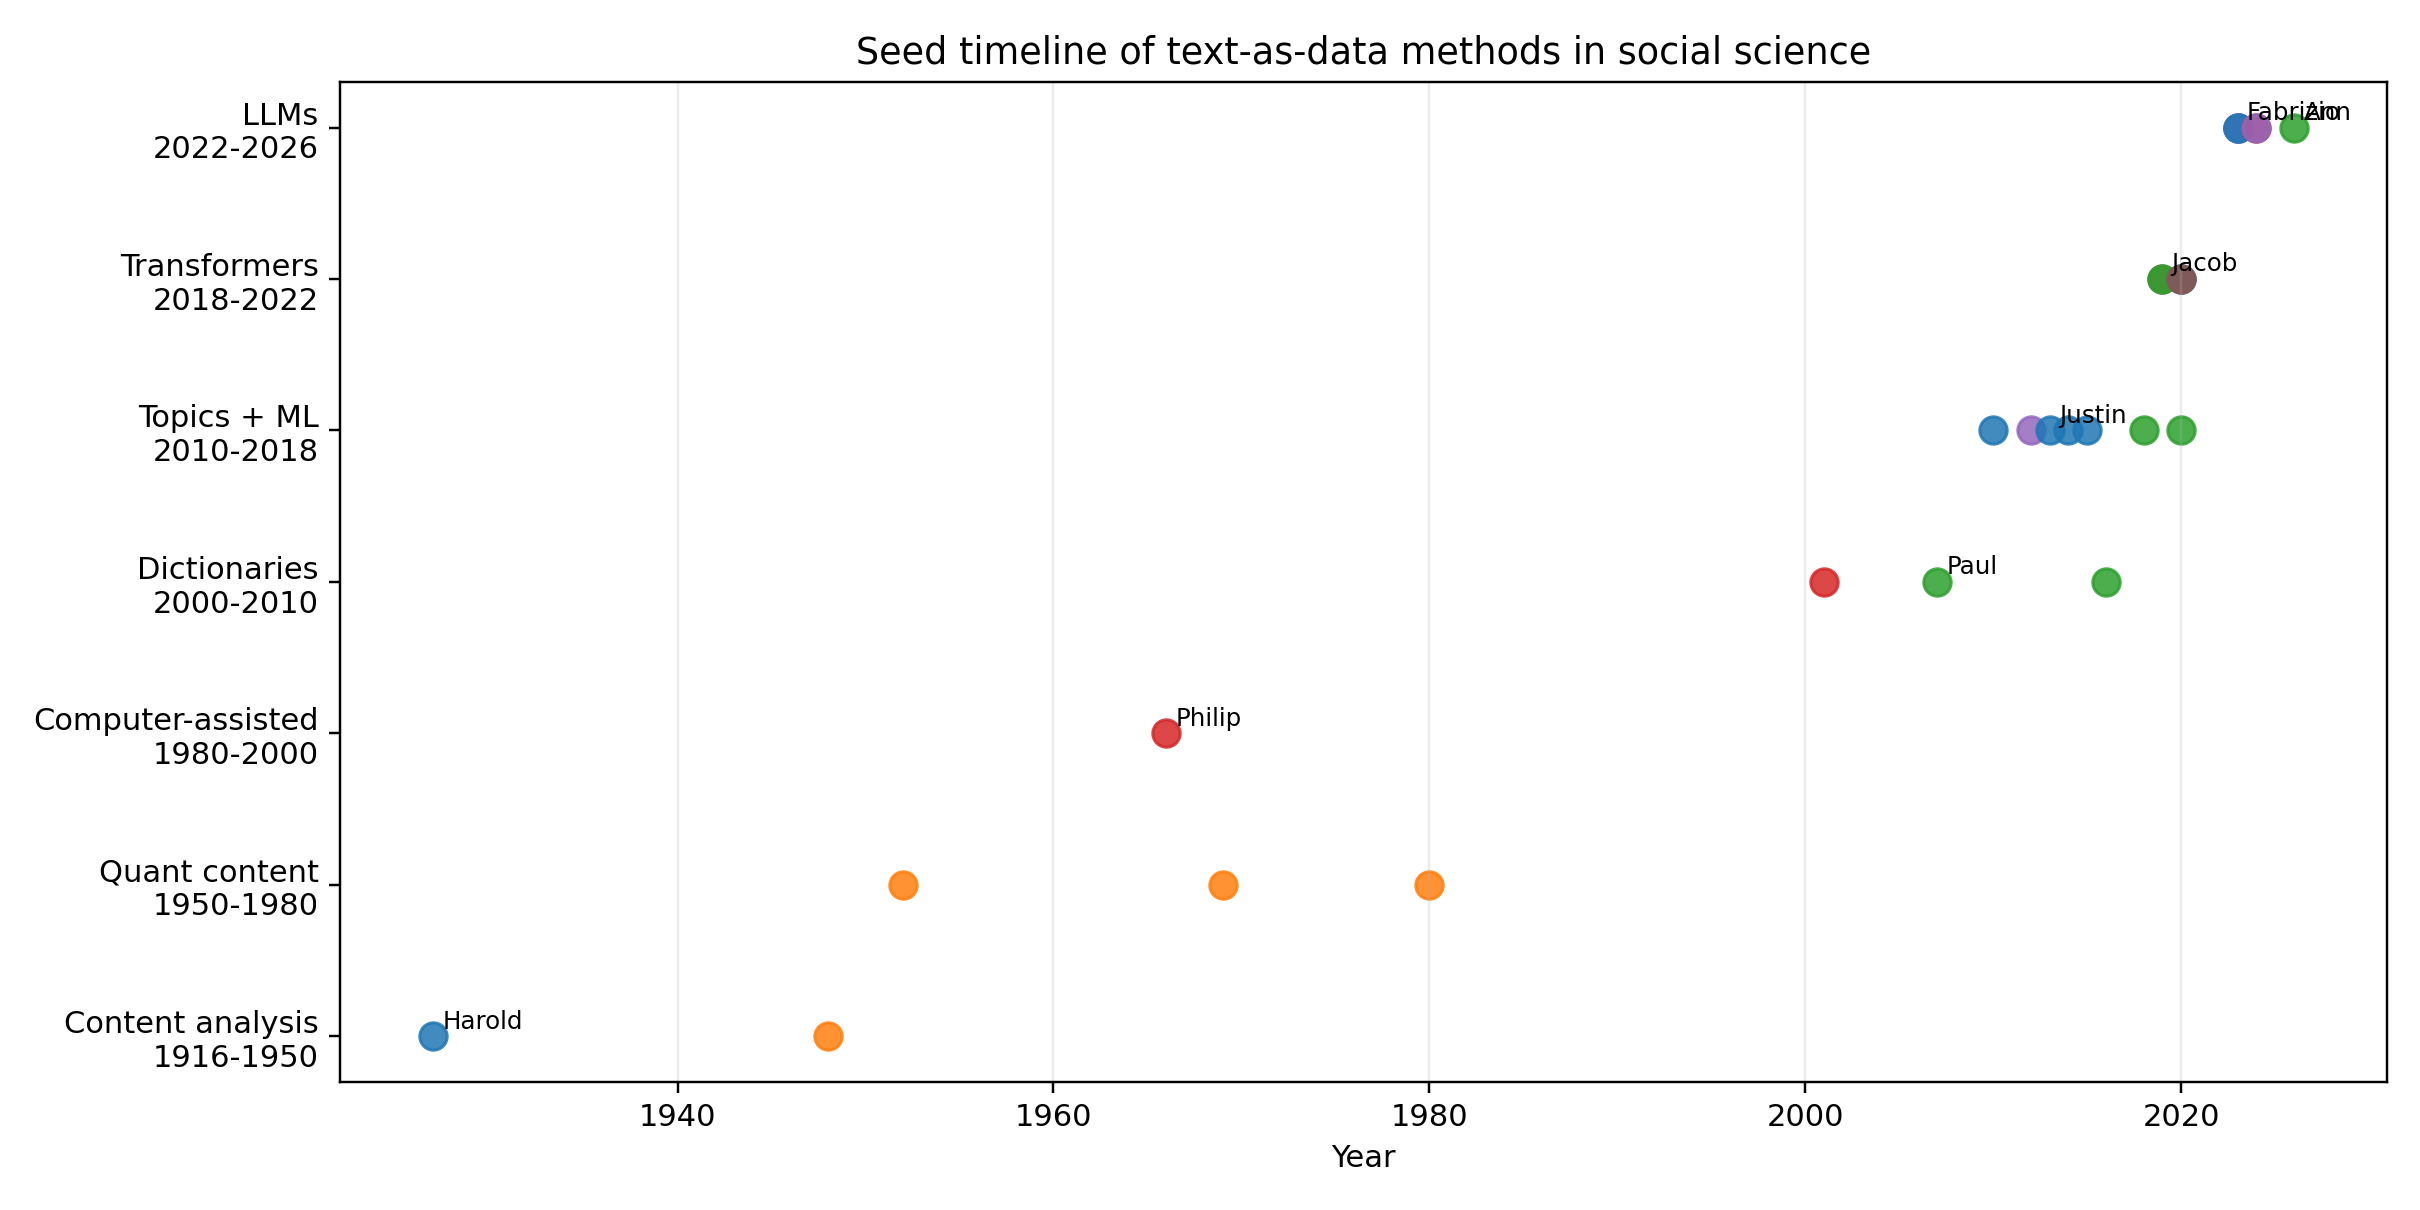
\includegraphics[width=0.95\linewidth]{../results/figures/timeline_seed.png}
\caption{Seed timeline of text-as-data methods}
\label{fig:timeline}
\end{figure}

\section{A Unified Taxonomy}

Text-as-data papers can be located along five dimensions: task, method, data type, discipline, and validation. Table \ref{tab:taxonomy} shows the method-task combinations in the seed database.

\begin{table}[ht]
\centering
\caption{Method-task taxonomy in the seed database}
\label{tab:taxonomy}
\begin{tabular}{llr}
\toprule
method\_family & task & n \\
\midrule
dictionary & measurement & 3 \\
dictionary & prediction & 1 \\
embeddings & measurement & 1 \\
large\_language\_model & classification & 3 \\
large\_language\_model & agenda & 2 \\
large\_language\_model & review & 1 \\
large\_language\_model & simulation & 1 \\
manual\_content\_analysis & measurement & 3 \\
manual\_content\_analysis & description & 1 \\
manual\_content\_analysis & theory & 1 \\
mixed\_methods & review & 3 \\
mixed\_methods & measurement & 1 \\
multilingual\_pipeline & measurement & 1 \\
supervised\_ml & measurement & 1 \\
topic\_modeling & discovery & 2 \\
topic\_modeling & measurement & 1 \\
topic\_modeling & prediction & 1 \\
transformer & classification & 1 \\
\bottomrule
\end{tabular}

\end{table}

The historical trend is not a simple replacement of old methods by new ones. Manual coding remains essential for validation. Dictionaries remain useful for transparency. Topic models remain valuable for exploration. Transformers and LLMs extend the toolkit, but they do not remove the need for theory, annotation, and external validation.

\begin{figure}[ht]
\centering
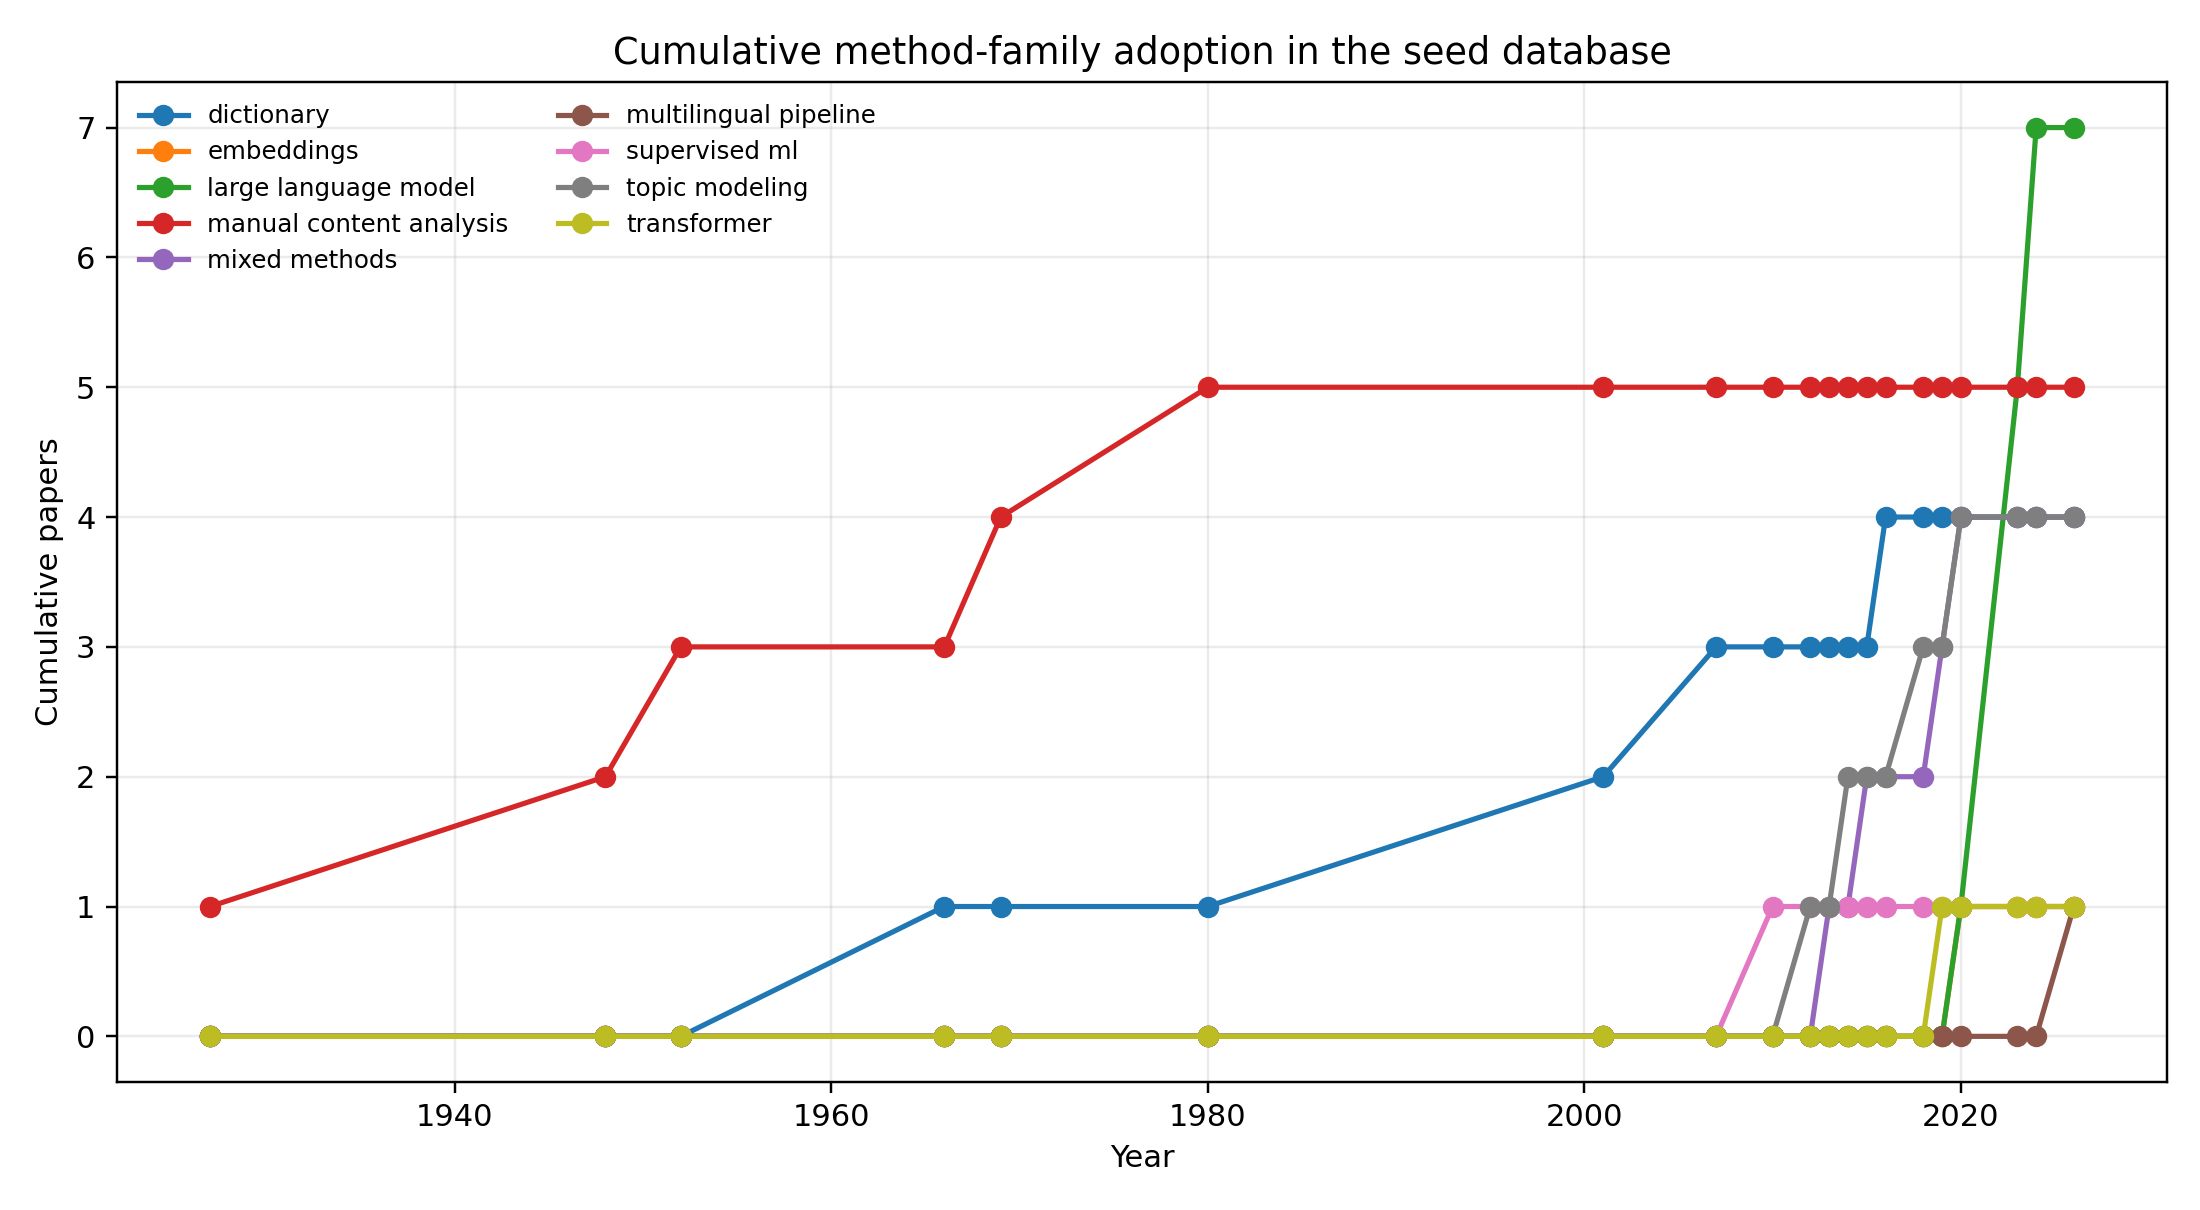
\includegraphics[width=0.9\linewidth]{../results/figures/method_adoption_seed.png}
\caption{Cumulative method-family adoption in the seed database}
\label{fig:method_adoption}
\end{figure}

\section{Disciplinary Adoption Patterns}

The seed database covers seven disciplinary areas. Table \ref{tab:disciplines} summarizes the distribution.

\begin{table}[ht]
\centering
\caption{Discipline coverage in the seed database}
\label{tab:disciplines}
\begin{tabular}{lr}
\toprule
discipline & n \\
\midrule
Political Science & 8 \\
Economics & 6 \\
Communication & 4 \\
Computational Social Science & 4 \\
Psychology & 3 \\
NLP & 2 \\
Law\_Economics & 1 \\
\bottomrule
\end{tabular}

\end{table}

Political science and communication adopted text analysis early through propaganda, speeches, and media studies. Psychology developed dictionary-based personality and affect measurement. Economics adopted text-as-data later, but now uses it heavily for uncertainty, sentiment, narratives, finance, and nowcasting. Computational social science has become the convergence layer, combining social questions with NLP methods.

\section{Geographic and Linguistic Gaps}

The seed database already shows the central problem: English-language research dominates. This will likely become even clearer in the full systematic review. The implication is substantive as well as technical. If most text-as-data research is English and US/European, then many public narratives, economic anxieties, and institutional discourses remain unmeasured.

\begin{figure}[ht]
\centering
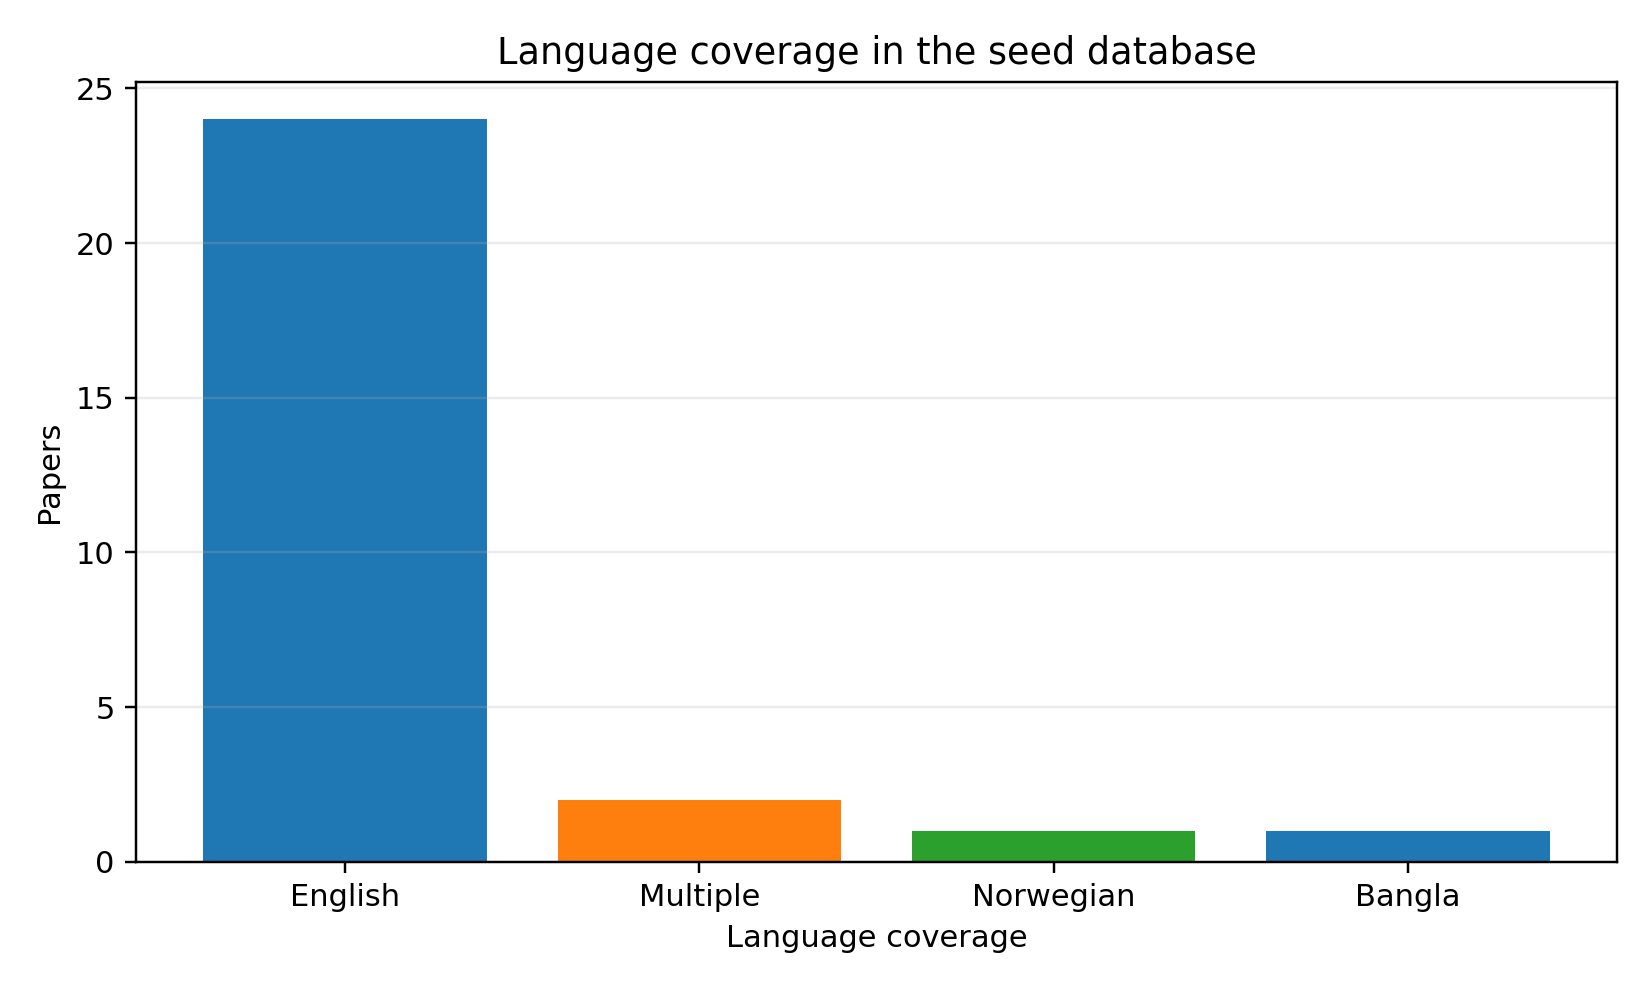
\includegraphics[width=0.72\linewidth]{../results/figures/language_gap_seed.png}
\caption{Language coverage in the seed database}
\label{fig:language_gap}
\end{figure}

The BENI research program is an example of the needed correction: local-language economic narrative measurement in Bangla for Bangladesh. It demonstrates how text-as-data infrastructure can move beyond English business media and into lower-resource language settings.

\section{Validation Standards Across Fields}

Validation practices vary sharply by field. Communication and political science emphasize manual coding and intercoder reliability. Economics often emphasizes external outcome validation and forecasting. NLP emphasizes benchmarks, but those benchmarks may be weak proxies for social-science validity. LLM-era work increasingly uses human--model comparison, but this is not sufficient unless tied to construct validity and downstream inference.

\begin{figure}[ht]
\centering
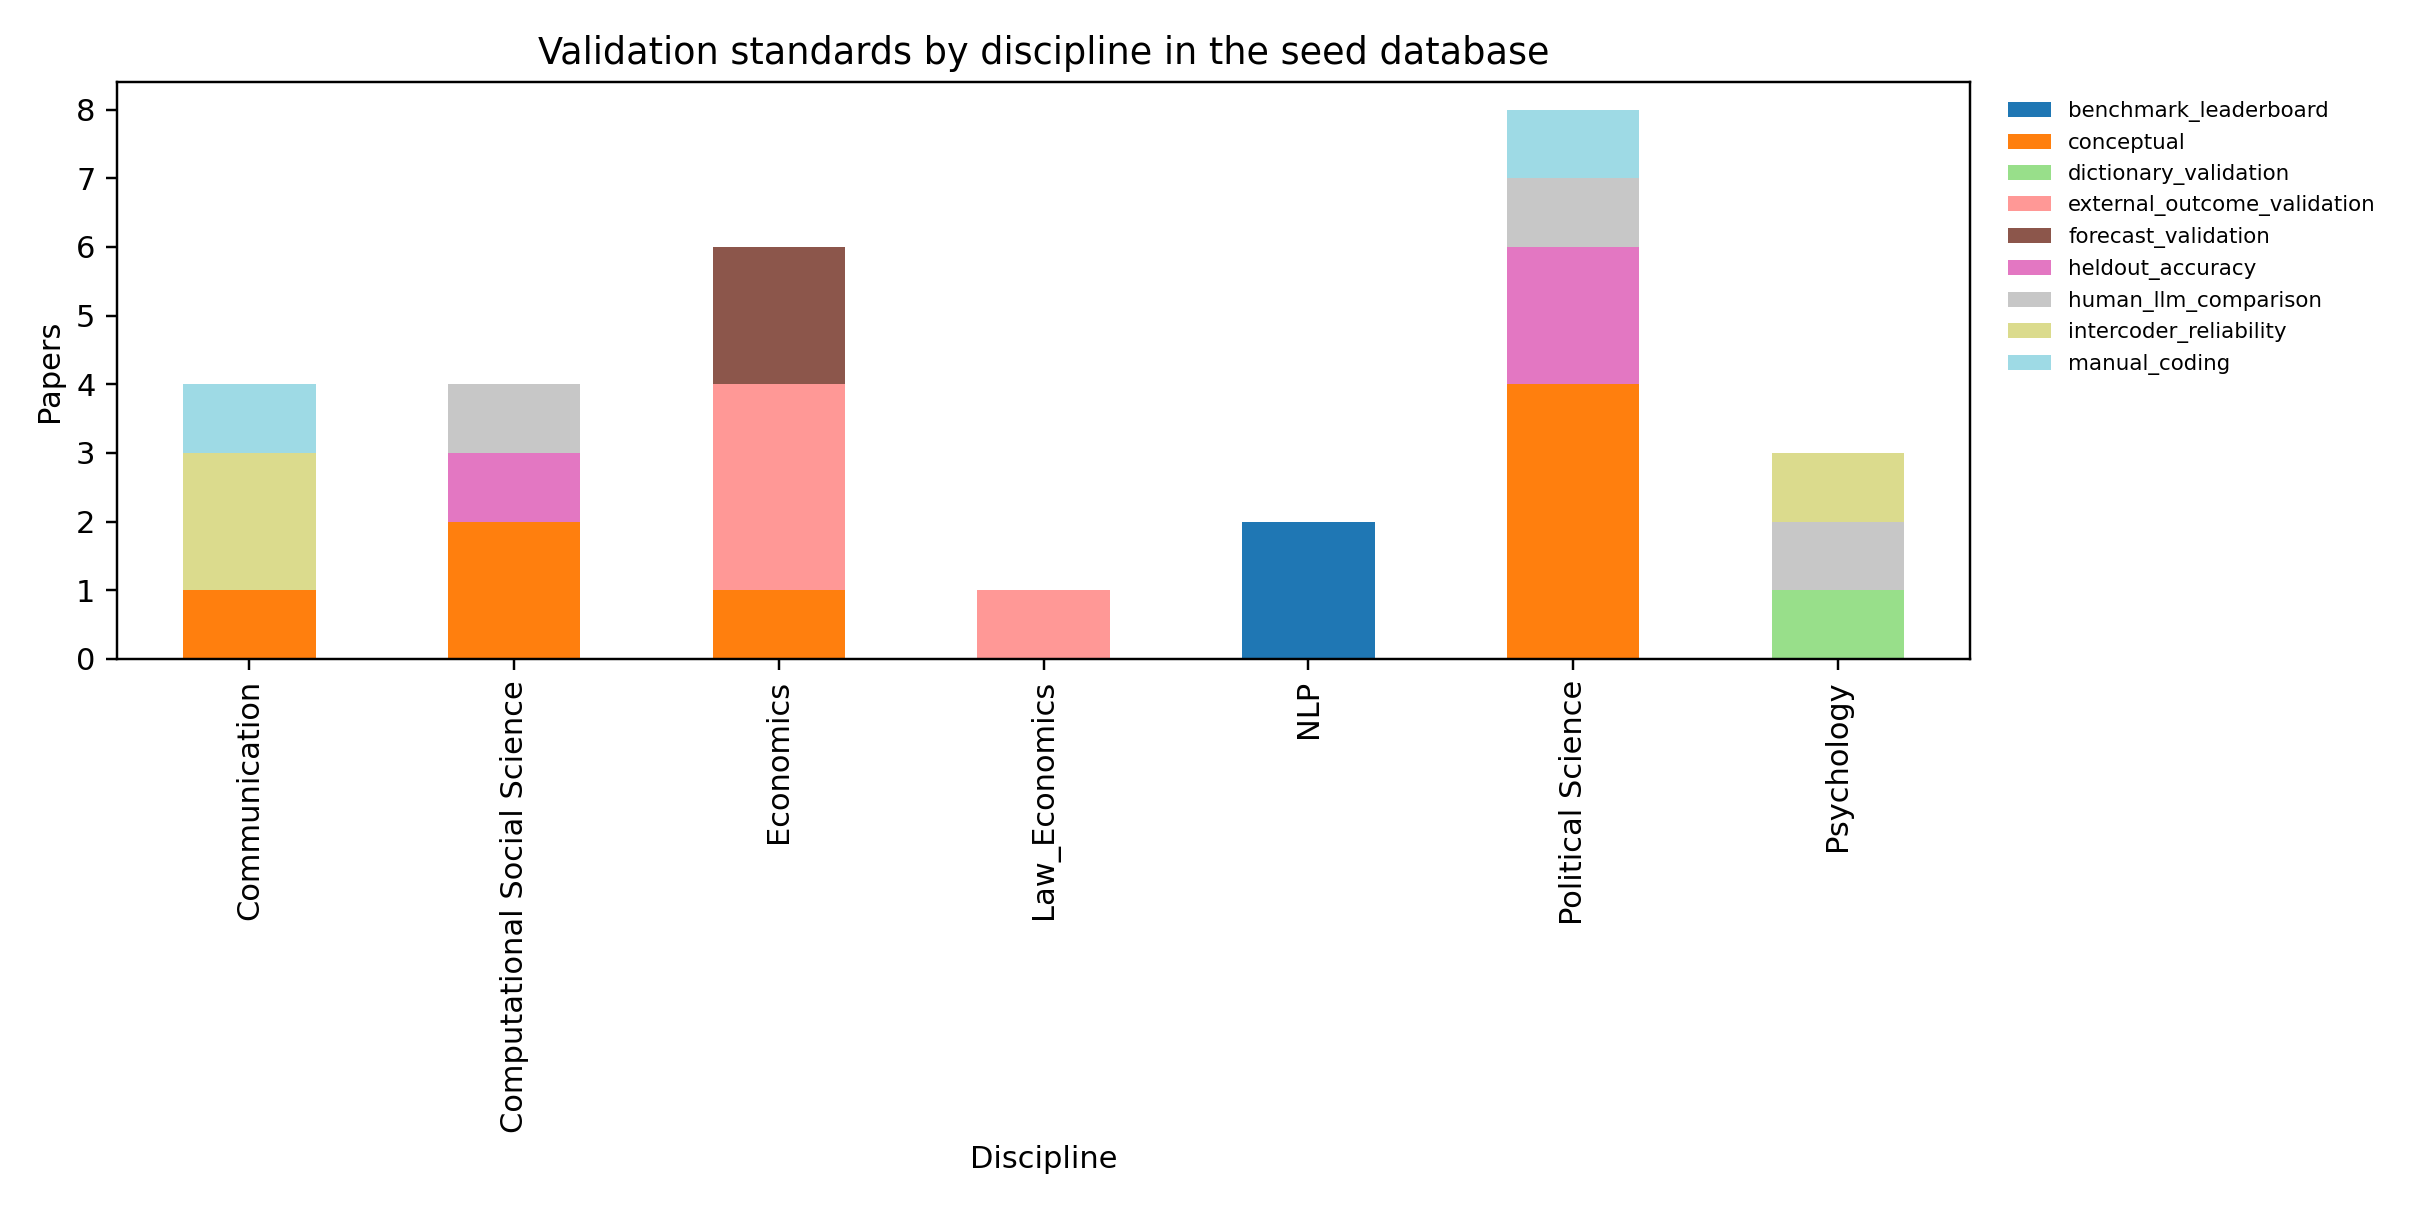
\includegraphics[width=0.95\linewidth]{../results/figures/validation_by_discipline.png}
\caption{Validation standards by discipline in the seed database}
\label{fig:validation}
\end{figure}

A minimal cross-disciplinary standard should include: clear construct definition, transparent annotation or prompt protocol, reliability checks, a baseline model, out-of-sample or external validation where possible, and explicit documentation of language/geographic scope.

\section{The LLM Revolution}

LLMs make text-as-data cheaper to start but harder to validate. They can annotate, summarize, translate, reason over long documents, and generate synthetic examples. They also introduce instability: model updates, hidden training data, prompt sensitivity, and hallucinated rationales.

\begin{figure}[ht]
\centering
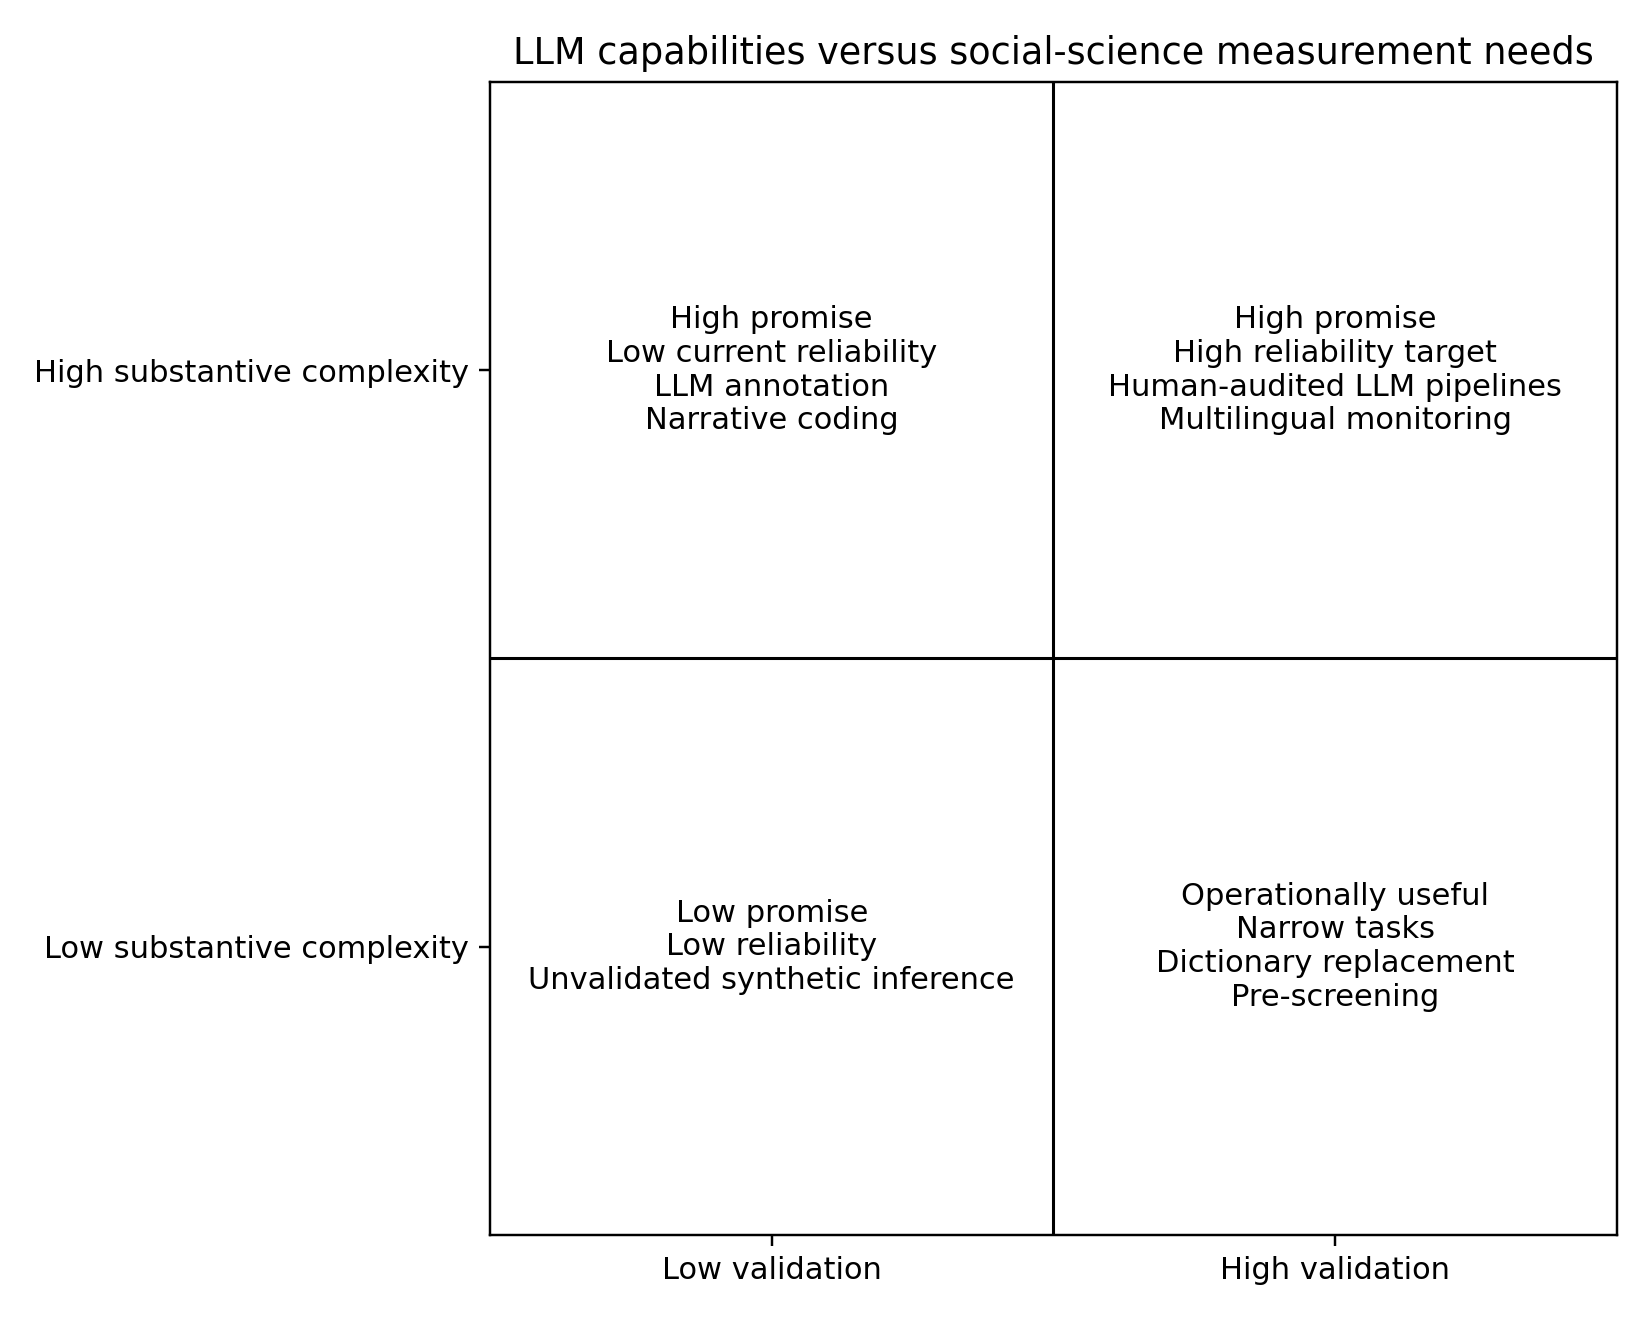
\includegraphics[width=0.75\linewidth]{../results/figures/llm_capability_matrix.png}
\caption{LLM capabilities versus social-science measurement needs}
\label{fig:llm_matrix}
\end{figure}

The best use of LLMs in social science is not fully automated measurement. It is human-audited measurement at scale: LLMs can pre-label, suggest categories, translate, flag ambiguous cases, and support iterative coding, but final inference still requires careful validation.

\section{Research Agenda for 2026--2036}

The next decade should focus on five priorities.

First, validation standards must become stronger and more portable across disciplines. Second, multilingual and non-Western corpora should become central rather than peripheral. Third, open-source pipelines and benchmark datasets should be developed for social-science tasks, not only NLP leaderboards. Fourth, journals should require clearer documentation of annotation, prompting, model versions, and replication packages. Fifth, LLMs should be integrated as auditable components in measurement pipelines, not treated as black-box replacements for research design.

The BENI case study fits this agenda. It builds a local-language economic narrative instrument, validates it against macroeconomic indicators, and then tests whether it has nowcasting value. This is the kind of measurement-plus-inference workflow that LLM-era text-as-data should pursue.

\section{Conclusion}

Text-as-data has matured from manual content analysis into a central infrastructure for empirical social science. The LLM era makes this infrastructure more powerful but also more fragile. The future of the field depends less on whether models become larger and more on whether researchers build valid, multilingual, reproducible, and theoretically grounded measurement systems.

\end{document}
